\documentclass[]{book}
\usepackage{lmodern}
\usepackage{amssymb,amsmath}
\usepackage{ifxetex,ifluatex}
\usepackage{fixltx2e} % provides \textsubscript
\ifnum 0\ifxetex 1\fi\ifluatex 1\fi=0 % if pdftex
  \usepackage[T1]{fontenc}
  \usepackage[utf8]{inputenc}
\else % if luatex or xelatex
  \ifxetex
    \usepackage{mathspec}
  \else
    \usepackage{fontspec}
  \fi
  \defaultfontfeatures{Ligatures=TeX,Scale=MatchLowercase}
\fi
% use upquote if available, for straight quotes in verbatim environments
\IfFileExists{upquote.sty}{\usepackage{upquote}}{}
% use microtype if available
\IfFileExists{microtype.sty}{%
\usepackage{microtype}
\UseMicrotypeSet[protrusion]{basicmath} % disable protrusion for tt fonts
}{}
\usepackage[unicode=true]{hyperref}
\hypersetup{
            pdftitle={Stat4: Binomiale data},
            pdfauthor={Team Toegepaste Biologie Venlo},
            pdfborder={0 0 0},
            breaklinks=true}
\urlstyle{same}  % don't use monospace font for urls
\usepackage{color}
\usepackage{fancyvrb}
\newcommand{\VerbBar}{|}
\newcommand{\VERB}{\Verb[commandchars=\\\{\}]}
\DefineVerbatimEnvironment{Highlighting}{Verbatim}{commandchars=\\\{\}}
% Add ',fontsize=\small' for more characters per line
\usepackage{framed}
\definecolor{shadecolor}{RGB}{248,248,248}
\newenvironment{Shaded}{\begin{snugshade}}{\end{snugshade}}
\newcommand{\KeywordTok}[1]{\textcolor[rgb]{0.13,0.29,0.53}{\textbf{{#1}}}}
\newcommand{\DataTypeTok}[1]{\textcolor[rgb]{0.13,0.29,0.53}{{#1}}}
\newcommand{\DecValTok}[1]{\textcolor[rgb]{0.00,0.00,0.81}{{#1}}}
\newcommand{\BaseNTok}[1]{\textcolor[rgb]{0.00,0.00,0.81}{{#1}}}
\newcommand{\FloatTok}[1]{\textcolor[rgb]{0.00,0.00,0.81}{{#1}}}
\newcommand{\ConstantTok}[1]{\textcolor[rgb]{0.00,0.00,0.00}{{#1}}}
\newcommand{\CharTok}[1]{\textcolor[rgb]{0.31,0.60,0.02}{{#1}}}
\newcommand{\SpecialCharTok}[1]{\textcolor[rgb]{0.00,0.00,0.00}{{#1}}}
\newcommand{\StringTok}[1]{\textcolor[rgb]{0.31,0.60,0.02}{{#1}}}
\newcommand{\VerbatimStringTok}[1]{\textcolor[rgb]{0.31,0.60,0.02}{{#1}}}
\newcommand{\SpecialStringTok}[1]{\textcolor[rgb]{0.31,0.60,0.02}{{#1}}}
\newcommand{\ImportTok}[1]{{#1}}
\newcommand{\CommentTok}[1]{\textcolor[rgb]{0.56,0.35,0.01}{\textit{{#1}}}}
\newcommand{\DocumentationTok}[1]{\textcolor[rgb]{0.56,0.35,0.01}{\textbf{\textit{{#1}}}}}
\newcommand{\AnnotationTok}[1]{\textcolor[rgb]{0.56,0.35,0.01}{\textbf{\textit{{#1}}}}}
\newcommand{\CommentVarTok}[1]{\textcolor[rgb]{0.56,0.35,0.01}{\textbf{\textit{{#1}}}}}
\newcommand{\OtherTok}[1]{\textcolor[rgb]{0.56,0.35,0.01}{{#1}}}
\newcommand{\FunctionTok}[1]{\textcolor[rgb]{0.00,0.00,0.00}{{#1}}}
\newcommand{\VariableTok}[1]{\textcolor[rgb]{0.00,0.00,0.00}{{#1}}}
\newcommand{\ControlFlowTok}[1]{\textcolor[rgb]{0.13,0.29,0.53}{\textbf{{#1}}}}
\newcommand{\OperatorTok}[1]{\textcolor[rgb]{0.81,0.36,0.00}{\textbf{{#1}}}}
\newcommand{\BuiltInTok}[1]{{#1}}
\newcommand{\ExtensionTok}[1]{{#1}}
\newcommand{\PreprocessorTok}[1]{\textcolor[rgb]{0.56,0.35,0.01}{\textit{{#1}}}}
\newcommand{\AttributeTok}[1]{\textcolor[rgb]{0.77,0.63,0.00}{{#1}}}
\newcommand{\RegionMarkerTok}[1]{{#1}}
\newcommand{\InformationTok}[1]{\textcolor[rgb]{0.56,0.35,0.01}{\textbf{\textit{{#1}}}}}
\newcommand{\WarningTok}[1]{\textcolor[rgb]{0.56,0.35,0.01}{\textbf{\textit{{#1}}}}}
\newcommand{\AlertTok}[1]{\textcolor[rgb]{0.94,0.16,0.16}{{#1}}}
\newcommand{\ErrorTok}[1]{\textcolor[rgb]{0.64,0.00,0.00}{\textbf{{#1}}}}
\newcommand{\NormalTok}[1]{{#1}}
\usepackage{longtable,booktabs}
\usepackage{graphicx,grffile}
\makeatletter
\def\maxwidth{\ifdim\Gin@nat@width>\linewidth\linewidth\else\Gin@nat@width\fi}
\def\maxheight{\ifdim\Gin@nat@height>\textheight\textheight\else\Gin@nat@height\fi}
\makeatother
% Scale images if necessary, so that they will not overflow the page
% margins by default, and it is still possible to overwrite the defaults
% using explicit options in \includegraphics[width, height, ...]{}
\setkeys{Gin}{width=\maxwidth,height=\maxheight,keepaspectratio}
\IfFileExists{parskip.sty}{%
\usepackage{parskip}
}{% else
\setlength{\parindent}{0pt}
\setlength{\parskip}{6pt plus 2pt minus 1pt}
}
\setlength{\emergencystretch}{3em}  % prevent overfull lines
\providecommand{\tightlist}{%
  \setlength{\itemsep}{0pt}\setlength{\parskip}{0pt}}
\setcounter{secnumdepth}{5}
% Redefines (sub)paragraphs to behave more like sections
\ifx\paragraph\undefined\else
\let\oldparagraph\paragraph
\renewcommand{\paragraph}[1]{\oldparagraph{#1}\mbox{}}
\fi
\ifx\subparagraph\undefined\else
\let\oldsubparagraph\subparagraph
\renewcommand{\subparagraph}[1]{\oldsubparagraph{#1}\mbox{}}
\fi
\usepackage{booktabs}

\title{Stat4: Binomiale data}
\author{Team Toegepaste Biologie Venlo}
\date{2020-03-13}

\usepackage{amsthm}
\newtheorem{theorem}{Theorem}[chapter]
\newtheorem{lemma}{Lemma}[chapter]
\newtheorem{corollary}{Corollary}[chapter]
\newtheorem{proposition}{Proposition}[chapter]
\newtheorem{conjecture}{Conjecture}[chapter]
\theoremstyle{definition}
\newtheorem{definition}{Definition}[chapter]
\theoremstyle{definition}
\newtheorem{example}{Example}[chapter]
\theoremstyle{definition}
\newtheorem{exercise}{Opdracht}[chapter]
\theoremstyle{remark}
\newtheorem*{remark}{Remark}
\newtheorem*{solution}{Solution}
\let\BeginKnitrBlock\begin \let\EndKnitrBlock\end
\begin{document}
\maketitle

{
\setcounter{tocdepth}{1}
\tableofcontents
}
\chapter*{Voorwoord}\label{voorwoord}
\addcontentsline{toc}{chapter}{Voorwoord}

Het afgelopen blok hebben jullie gewerkt met responsvariabelen die van
het niveau interval/ratio en continue zijn, op een hoofdstuk na:
survival analysis.

Survivaldata is een duidelijk voorbeeld van binomiale data. Het kan twee
waardes aannemen: dood/levend, heel/kapot, etc. In dit blok gaan we
verder met binomiale data (hoofdstuk 1 en 2).

Verder gaan we aan de slag met frequentiedata (hoofstuk 3). Een
voorbeeld van frequentiedata heb je al verzameld en geanalyseerd in jaar
1 (krekelpracticum) en mogelijk ook tijdens je eigen project in blok 2
(diergedrag).

Hoofstuk 4 en 5 gaan over multivariate technieken. Dan heb je te maken
met meerdere responsvariabelen.

We eindigen dit blok met een overzicht van alle toetsen die jullie gehad
hebben. Hiermee hopen we dat jullie voorbereid zijn op dataverwerking in
jaar 3 en 4. Dan moeten jullie het namelijk zelf kunnen.

\chapter{Binomiale verdeling: toets op
fractie}\label{binomiale-verdeling-toets-op-fractie}

\BeginKnitrBlock{ABD}
Lees chapter 7 (\emph{Analysing proportions})
\EndKnitrBlock{ABD}

De binomiale verdeling werd al in de 17\textsuperscript{de} eeuw
uitgebreid onderzocht. In die tijd was het spel kop-en-munt razend
populair. Je moest gokken, van een x-aantal munten, hoeveel kop of munt
je zou krijgen. Doe je dat spelletje met één munt, dan is het niet zo
moeilijk. De kans op kop of munt is gelijk (tenminste bij een
``eerlijke'' munt).

Voor een grotere serie, moet je gaan rekenen. Doe je dit voor n=2, dan
zijn dit de opties:

\begin{tabular}{l|l|r}
\hline
munt1 & munt2 & aantal\_kop\\
\hline
munt & munt & 0\\
\hline
munt & kop & 1\\
\hline
kop & munt & 1\\
\hline
kop & kop & 2\\
\hline
\end{tabular}

Kans op 0x kop = 1/4, kans op 1x kop = 2/4 en kans op 2x kop = 1/4.

Bij grotere n is dat aardig wat rekenwerk. Gelukkig heeft R daar een
functie voor. Als voorbeeld de kans dat je 2x kop hebt bij een serie van
2 muntjes:

\begin{Shaded}
\begin{Highlighting}[]
\KeywordTok{dbinom}\NormalTok{(}\DataTypeTok{x=}\DecValTok{2}\NormalTok{, }\DataTypeTok{size =} \DecValTok{2}\NormalTok{, }\DataTypeTok{prob =} \FloatTok{0.5}\NormalTok{)}
\end{Highlighting}
\end{Shaded}

\begin{verbatim}
## [1] 0.25
\end{verbatim}

\BeginKnitrBlock{exercise}
\protect\hypertarget{exr:kop-of-munt}{}{\label{exr:kop-of-munt} }Bereken de
volgende kansen:

\begin{itemize}
\tightlist
\item
  1 keer kop bij n=2
\item
  4 keer kop bij n=8
\item
  8 keer kop bij n=16
\end{itemize}

Bedenk waarom de kans afneemt?
\EndKnitrBlock{exercise}

\section{Betrouwbaarheidsinterval}\label{betrouwbaarheidsinterval}

In het geval van kop-en-munt weet je (ongeveer) de theoretische kans
(\emph{probability}), je gaat er vanuit dat die 0,5. De kans wordt
weergegeven met de letter \textbf{p} (niet te verwarren met hetzelfde
symbool voor de overschrijdingskans van onder de
H\textsubscript{0}-hypothese). Meestal wordt er gesproken van kans op
\textbf{succes}, waarbij je zelf aangeeft welke van de twee waardes je
succes noemt (kop of munt).

Vaak weet je \textbf{p} niet, en schat je die vanuit een steekproef,
weergegeven met \(\hat{p}\).

Net als bij de normale verdeling, kan je het betrouwbaarheidsinterval
berekenen van je schatter. Bij de normale verdeling gaat het vaak om het
gemiddelde, bij de binomiale data gaat het om \(\hat{p}\).

Ook hier geldt weer dat de schatting alleen betrouwbaar is als de
daadwerkelijke verdeling de regels van je theoretische verdeling volgt.
Voor de binomiale verdeling geldt:

\begin{itemize}
\tightlist
\item
  Het aantal steekproeven (n) staat vast (dus bijv. 10x kop-of-munt)
\item
  De steekproeven zijn onafhankelijk van elkaar
\item
  De kans op succes (p) is gelijk voor iedere steekproef
\end{itemize}

Wanneer we ervan uit kunnen gaan dat de verdeling aan bovenstaande
voorwaarden voldoet, kunnen we een betrouwbaarheidsinterval uitrekenen.

Hoe doe je dat in R?

\begin{Shaded}
\begin{Highlighting}[]
\KeywordTok{library}\NormalTok{(Hmisc)}
\KeywordTok{binconf}\NormalTok{(x, n, }\DataTypeTok{alpha=}\FloatTok{0.05}\NormalTok{)}
\end{Highlighting}
\end{Shaded}

waarbij x het aantal successen is, en n het aantal steekproeven. In het
geval van voorbeel 7.3 uit het boek:

\begin{Shaded}
\begin{Highlighting}[]
\KeywordTok{library}\NormalTok{(Hmisc)}
\KeywordTok{binconf}\NormalTok{(}\DataTypeTok{x=}\DecValTok{30}\NormalTok{, }\DataTypeTok{n=}\DecValTok{87}\NormalTok{, }\DataTypeTok{alpha=}\FloatTok{0.05}\NormalTok{)}
\end{Highlighting}
\end{Shaded}

\begin{verbatim}
##   PointEst     Lower     Upper
##  0.3448276 0.2534266 0.4493523
\end{verbatim}

Zoals je ziet is \texttt{binconf()} een functie uit de package Hmisc.

\BeginKnitrBlock{exercise}
\protect\hypertarget{exr:Hmisc}{}{\label{exr:Hmisc} }Package Hmisc

\begin{itemize}
\tightlist
\item
  installeer de package Hmisc
\end{itemize}
\EndKnitrBlock{exercise}

\BeginKnitrBlock{exercise}
\protect\hypertarget{exr:dobbelsteen1}{}{\label{exr:dobbelsteen1}
}Betrouwbare dobbelsteen

Stel, je werpt 20 keer met een dobbelsteen en gooit 0 keer 6.

\begin{itemize}
\tightlist
\item
  Bereken het betrouwbaarheidsinterval van de kans op 6 op basis van
  bovenstaande steekproef.
\item
  Verwacht je dat de dobbelsteen ``zuiver'' is (kans op iedere waarde is
  gelijk)?
\end{itemize}
\EndKnitrBlock{exercise}

\section{De binomiale toets}\label{de-binomiale-toets}

Je kan ook testen of de gevonden \(\hat{p}\) afwijkt van een
theoretische waarde. In het geval van de vorige opgave, over de
dobbelsteen, kan je testen of p\textless{} 1/6:

\begin{Shaded}
\begin{Highlighting}[]
\KeywordTok{binom.test}\NormalTok{(}\DecValTok{0}\NormalTok{, }\DecValTok{20}\NormalTok{, }\DataTypeTok{p=}\DecValTok{1}\NormalTok{/}\DecValTok{6}\NormalTok{, }\DataTypeTok{alternative =} \StringTok{"less"}\NormalTok{)}
\end{Highlighting}
\end{Shaded}

\begin{verbatim}
## 
##  Exact binomial test
## 
## data:  0 and 20
## number of successes = 0, number of trials = 20, p-value = 0.02608
## alternative hypothesis: true probability of success is less than 0.1666667
## 95 percent confidence interval:
##  0.0000000 0.1391083
## sample estimates:
## probability of success 
##                      0
\end{verbatim}

De functie \texttt{binom.test()} berekent de \textbf{exacte} kans op het
voorkomen van de gegeven, of meer extremere uitkomst bij een bepaalde p
(in dit geval 1/6). Net als bij de t-toets kan je aangeven of je
eenzijdig, danwel tweezijdig wilt toetsen.

De hypotheses die bij bovenstaande code horen zijn:

\begin{itemize}
\tightlist
\item
  H\textsubscript{0}: \(p = 1/6\) of, meer formeel, \(p \geq 1/6\)
\item
  H\textsubscript{1}: \(p < 1/6\)
\end{itemize}

\textbf{NB}: de binomiale test geeft ook een betrouwbaarheidsinterval,
maar deze is gebaseerd op de F-verdeling (bij grote steekproeven volgt
een binomiale verdeling min of meer een normale verdeling). Zoals je kan
lezen in het boek, kan je beter een andere methode gebruiken: de
Agresti-Coull-methode (``Wilson interval''). Dat is de standaardmethode
in d functie \texttt{binconf()}.

\BeginKnitrBlock{exercise}
\protect\hypertarget{exr:dobbelsteen2}{}{\label{exr:dobbelsteen2}
}Dobbelsteen

Je gooit met een dobbelsteen 6 keer, en je gooit telkens 4. Je wilt
testen of de dobbelsteen afwijkt t.o.v. een zuivere dobbelsteen.

\begin{itemize}
\tightlist
\item
  Geef de hypotheses
\item
  Bereken de overschrijdingskans.
\end{itemize}
\EndKnitrBlock{exercise}

\section{Verschiltoets voor fracties}\label{verschiltoets-voor-fracties}

Soms wil je een fractie niet testen ten opzichte van een theoretische
waarde, maar juist met een andere steekproef.

Stel dat je de kans op 6 voor twee dobbelstenen wilt vergelijken. Je
vermoedt dat ze verschillen van elkaar. Met de ene dobbelsteen gooi je
100 keer, en je krijgt 12x zes, en met de andere dobbelsteen gooi je 80
keer en je krijgt 20x zes. Je hypotheses zijn:

\begin{itemize}
\tightlist
\item
  H\textsubscript{0}: \(p_{1} \neq p_{2}\)
\item
  H\textsubscript{1}: \(p_{1} = p_{2}\)
\end{itemize}

Met de volgende functie test dit in R:

\begin{Shaded}
\begin{Highlighting}[]
\NormalTok{succes =}\StringTok{ }\KeywordTok{c}\NormalTok{(}\DecValTok{12}\NormalTok{, }\DecValTok{20}\NormalTok{, }\DecValTok{5}\NormalTok{)}
\NormalTok{n =}\StringTok{ }\KeywordTok{c}\NormalTok{(}\DecValTok{100}\NormalTok{, }\DecValTok{80}\NormalTok{, }\DecValTok{60}\NormalTok{)}
\KeywordTok{prop.test}\NormalTok{(succes, n)}
\end{Highlighting}
\end{Shaded}

\begin{verbatim}
## 
##  3-sample test for equality of proportions without continuity
##  correction
## 
## data:  succes out of n
## X-squared = 8.8382, df = 2, p-value = 0.01204
## alternative hypothesis: two.sided
## sample estimates:
##     prop 1     prop 2     prop 3 
## 0.12000000 0.25000000 0.08333333
\end{verbatim}

De functie \texttt{prop.test()} heeft als input een vector met de
aantallen succes voor de verschillende objecten (je kan de toets met
meer dan twee groepen uitvoeren ). Als toets wordt een chi-kwadraattoets
uitgevoerd. Daarover leer je meer in hoofdstuk 2.

\section{Opgaven}\label{opgaven}

Gebruik voor de volgende opgaven R.

In het boek wordt ervan uitgegaan dat je per mogelijke uitkomst
(bijvoorbeeld 5 resistente stammen in opgave 1) de kans berekent met je
rekenmachine. Dat kan natuurlijk gemakkelijker in R. Met de functie
\texttt{dbinom(x,\ n,\ prob)} kan je de exacte kans berekenen. In het
geval van opgave 1c: \texttt{dbinom(x=5,\ n=7,\ prob=0.3)}, of nog
korter: \texttt{dbinom(5,\ 7,\ 0.3)}.

Maar als je de kans op minstens of maximaal x successen wilt berekenen,
dan kan dat natuurlijk ook met \texttt{binom.test()}. Voor opgave 1e
krijg je dan:
\texttt{binom.test(x=5,\ n=7,\ p=0.3,\ alternative="greater")}.

Wordt er gevraagd naar een confidence interval via de
Agresti-Coull-methode: R doet dat automatisch met de functie
\texttt{binconf()}.

\BeginKnitrBlock{exercise}
\protect\hypertarget{exr:PP07}{}{\label{exr:PP07} }Practise Problems,
chapter 7

Los de volgende Practise problems op:

\begin{itemize}
\tightlist
\item
  1 t/m 4.
\item
  6 t/m 9

  \EndKnitrBlock{exercise}
\end{itemize}

\BeginKnitrBlock{exercise}
\protect\hypertarget{exr:verschiltoetsfrac}{}{\label{exr:verschiltoetsfrac}
}Zaadbehandeling

In een onderzoek worden 120 ontkiemde zaden behandeld met 18 uur donker
/ 6 uur licht (behandeling A) en 80 ontkiemde zaden met 12 uur licht /
12 uur donker (behandeling B). Na precies 2 weken werd er gekeken
hoeveel zaden volledig tot groei gekomen waren. Bij behandeling A waren
dat er 92 van de 120 en bij behandeling B waren dat er 48 van de 80.

\begin{itemize}
\tightlist
\item
  Toets met \(\alpha = 0,05\) de hypothese dat behandeling A beter werkt
  dan behandeling B.
\end{itemize}
\EndKnitrBlock{exercise}

\BeginKnitrBlock{exercise}
\protect\hypertarget{exr:medicijn}{}{\label{exr:medicijn} }Medicijn
\EndKnitrBlock{exercise}

Een fabrikant beweert dat zijn medicijn (A) in 70\% van de behandelingen
bij paarden effectief is. Een onderzoeker vergelijkt A met een andere
medicijn (B) en vindt de volgende resultaten:

\begin{tabular}{l|r|r}
\hline
Soort medicijn & wel effectief & niet effectief\\
\hline
A & 19 & 11\\
\hline
B & 19 & 6\\
\hline
\end{tabular}

De onderzoeker meent dat de door de fabrikant aangegeven percentage van
70\% te hoog is.

\begin{itemize}
\tightlist
\item
  Is dit op basis van bovenstaande steekproef met een zekerheid van 95\%
  te beweren? Formuleer de hypothese en voer een toets uit en eindig met
  een duidelijke conclusie
\item
  Toets met een foutmarge van \(\alpha =0,05\) de bewering dat medicijn
  B beter werkt dan
\end{itemize}

\chapter{Logistische regressie}\label{logistische-regressie}

\BeginKnitrBlock{ABD}
\begin{itemize}
\tightlist
\item
  Lees paragraph 9.2 (\emph{Estimating})
\item
  Lees paragraph 17.9 (\emph{Logistic regression: fitting a binary
  response variable})
\end{itemize}
\EndKnitrBlock{ABD}

In het vorige hoofdstuk heb je kennis gemaakt met binaire data
(dood/levend, etc.). Je kan deze kans beschrijven als een kansproces met
de kans p op ``succes''. Je hebt al geleerd om te bepalen wat het
betrouwbaarheidsinterval is van de geschatte p uit een steekproef en of
de p van twee steekproeven significant van elkaar verschillen.

Maar er zijn meer onderzoeksvragen mogelijk. Ter illustratie een
voorbeeld over tomaten:

Een tomatenteler onderzoekt of de tomatenoogst eerder kan, zonder dat de
tomaten onrijp worden geoogst. Het volgende experiment wordt uitgevoerd:

\begin{itemize}
\tightlist
\item
  Bij zes planten worden de tomaten 10 dagen eerder dan normaal geoogst.
\item
  Bij vier andere planten worden de tomaten 5 dagen eerder geoogst.
\item
  Bij zes planten worden de tomaten op de standaardtijd geoogst.
\end{itemize}

Vervolgens wordt gekeken hoeveel van de geplukte tomaten, per tijdstip,
rijp zijn:

\begin{tabular}{l|r|r}
\hline
  & onrijp & rijp\\
\hline
-10 & 5 & 1\\
\hline
-5 & 1 & 3\\
\hline
0 & 1 & 5\\
\hline
\end{tabular}

Zulke data kan je mooi presenteren in een mozaiekplot (In het Engels
\emph{mosaic plot} geheten):

\begin{Shaded}
\begin{Highlighting}[]
\KeywordTok{library}\NormalTok{(ggmosaic)}

\NormalTok{tomaat %>%}\StringTok{ }
\StringTok{  }\KeywordTok{ggplot}\NormalTok{() +}
\StringTok{  }\KeywordTok{geom_mosaic}\NormalTok{(}\KeywordTok{aes}\NormalTok{(}\DataTypeTok{x=}\KeywordTok{product}\NormalTok{(tijd), }\DataTypeTok{fill =} \NormalTok{rijp)) +}
\StringTok{  }\KeywordTok{scale_fill_manual}\NormalTok{(}\DataTypeTok{values =} \KeywordTok{c}\NormalTok{(}\StringTok{"green"}\NormalTok{, }\StringTok{"red"}\NormalTok{)) +}
\StringTok{  }\KeywordTok{xlab}\NormalTok{(}\StringTok{"tijd (dagen voor oogstijd)"}\NormalTok{) +}
\StringTok{  }\KeywordTok{ylab}\NormalTok{(}\StringTok{"fractie rijp"}\NormalTok{) +}
\StringTok{  }\KeywordTok{theme}\NormalTok{(}\DataTypeTok{legend.position =} \StringTok{"none"}\NormalTok{)}
\end{Highlighting}
\end{Shaded}

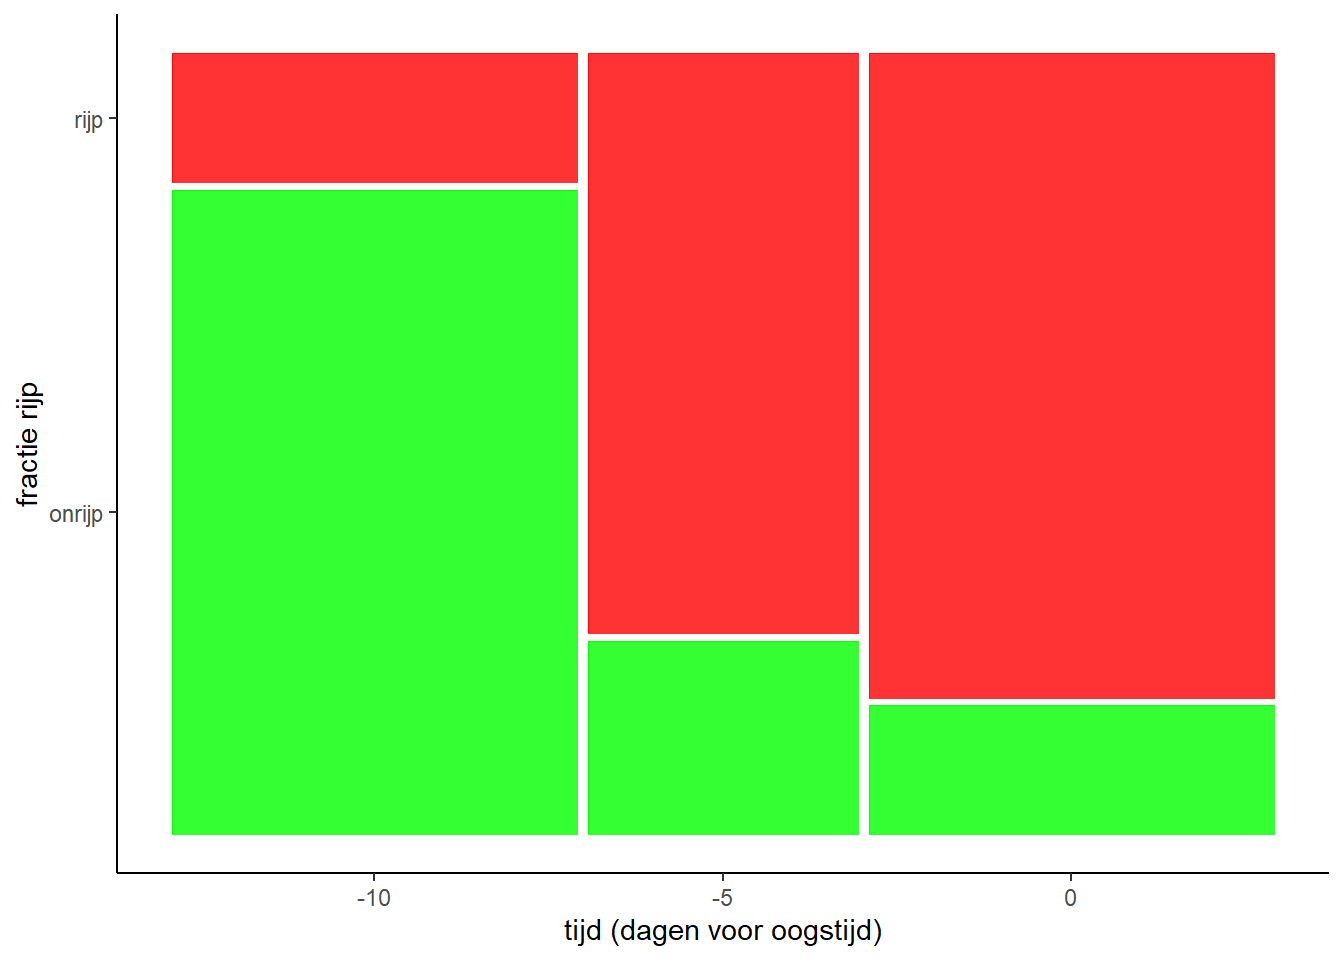
\includegraphics{hfst2_logregr_files/figure-latex/unnamed-chunk-3-1.pdf}

Kenmerk van een mozaiekplot is dat op de y-as en x-as af te lezen welke
fractie in welke categorie gevonden is. Zie ook in het boek blz. 40-41.
Voor het creëren van zulke plots heb je de package \textbf{ggmosaic}
nodig. NB: de variabele voor de x-as moet opgegeven worden als
\texttt{product(variabele)}.

De code voor bovenstaande figuur heeft wel wat extra code om de figuur
op te leuken:

\begin{itemize}
\tightlist
\item
  \texttt{scale\_fill\_manual(values\ =\ c("green",\ "red"))\ +}:
  handmatig kleuren kiezen
\item
  \texttt{xlab("tijd\ (dagen\ voor\ oogstijd)")\ +}: label voor x-as
  definiëren
\item
  \texttt{ylab("fractie\ rijp")\ +}: label voor y-as definiëren
\item
  \texttt{theme(legend.position\ =\ "none")}: legenda niet laten zien
\end{itemize}

\BeginKnitrBlock{exercise}
\protect\hypertarget{exr:ggmosaic}{}{\label{exr:ggmosaic} }ggmosaic

\begin{itemize}
\tightlist
\item
  Installeer de package ggmosiac
\item
  Maak van je krekeldata een mozaiekplot (weliswaar geen bonomiale data,
  maar mozaiekplot werkt ook voor zulke data)
\end{itemize}
\EndKnitrBlock{exercise}

In de volgende paragrafen gaan we hypothesetoetsen voor binomiale data
uitvoeren.

\section{Generalized Linear Model}\label{generalized-linear-model}

De responsdata is nu binomiaal verdeeld, dus je kan geen gewoon
\emph{General Linear Model} toepassen. Daarvoor in de plaats gebruiken
we het \emph{Generalized Linear Model}, met de functie in R:
\texttt{glm()}.

Verschil met de functie \texttt{lm()} is dat je nu kan aangeven wat voor
soort data je hebt. In dit geval hebben we te maken met binomiale data:

\begin{Shaded}
\begin{Highlighting}[]
\KeywordTok{glm}\NormalTok{(respons~verklarende, }\DataTypeTok{family =} \KeywordTok{binomial}\NormalTok{())}
\end{Highlighting}
\end{Shaded}

Met deze informatie zet de glm de responsveriabele om naar
\textbf{log-odds}, dat is een alternatieve manier om kans weer te geven:

\[\log{\frac{p}{1-p}}\]

De fractie \(\frac{p}{1-p}\) wordt de \textbf{odd} genoemd en komt
misschien raar over, maar is iets wat jullie waarschijnlijk allemaal
ooit hebben gebruikt: ``die kans is fifty-fifty'' of ``tien tegen een''.

\BeginKnitrBlock{exercise}
\protect\hypertarget{exr:unnamed-chunk-5}{}{\label{exr:unnamed-chunk-5} }Odd

\begin{itemize}
\tightlist
\item
  Welke odd-waarde heeft de kans ``fifty-fifty is''?
\item
  Welke odd-waarde heeft een kans van tien tegen een?
\item
  Welke odd-waarde heeft rijpheid van tomaten bij 10 dagen voor
  oogsttijd?
\end{itemize}
\EndKnitrBlock{exercise}

\section{ANOVA met binomiale data}\label{anova-met-binomiale-data}

Stel, we willen testen of tijdstip van oogsten echt een effect heeft op
de rijpheid, dan krijgen we de volgende hypotheses:

\begin{itemize}
\tightlist
\item
  H\textsubscript{0}: alle tijdstippen hebben gelijke kans op rijpheid
\item
  H\textsubscript{1}: minstens een verschil in kans op rijpheid tussen
  tijdstippen
\end{itemize}

Dat klinkt als een \emph{one-way ANOVA}, maar dan met binomiale data. En
dat is het ook. Om het \emph{generalized linear model} uit te voeren,
moet de responsvariabele in de vorm 0 of 1 zijn. In dit geval zijn het
twee categoriën in de vorm van tekst (``rijp'' en ``onrijp''). Om die om
te zetten gebruiken we de functien\texttt{recode()}:

\begin{Shaded}
\begin{Highlighting}[]
\NormalTok{tomaat_num <-}\StringTok{ }\NormalTok{tomaat %>%}\StringTok{ }
\StringTok{  }\KeywordTok{mutate}\NormalTok{(}\DataTypeTok{rijp =} \KeywordTok{recode}\NormalTok{(rijp, }\StringTok{"onrijp"} \NormalTok{=}\StringTok{ }\DecValTok{0}\NormalTok{, }\StringTok{"rijp"} \NormalTok{=}\StringTok{ }\DecValTok{1}\NormalTok{))}
\end{Highlighting}
\end{Shaded}

Met de functie \texttt{mutate()} definieer je een nieuwe variabele (in
dit geval weer rijp genoemd). Met \texttt{recode()} zet je de variabele
rijp om van tekst naar 0-en en 1-en. En natuurlijk uitgevoerd in een
\emph{pipeline}.

Volgende stap is om het \emph{generalized linear model} uit te voeren:

\begin{Shaded}
\begin{Highlighting}[]
\NormalTok{fit <-}\StringTok{ }\KeywordTok{glm}\NormalTok{(rijp~}\KeywordTok{factor}\NormalTok{(tijd), }\DataTypeTok{family =} \KeywordTok{binomial}\NormalTok{(), }\DataTypeTok{data =} \NormalTok{tomaat_num)}
\end{Highlighting}
\end{Shaded}

En vervolgens een soort van ANOVA-tabel, dat doen we nu met de functie
\texttt{Anova()} uit de package car:

\begin{Shaded}
\begin{Highlighting}[]
\KeywordTok{library}\NormalTok{(car)}
\KeywordTok{Anova}\NormalTok{(fit)}
\end{Highlighting}
\end{Shaded}

\begin{verbatim}
## Analysis of Deviance Table (Type II tests)
## 
## Response: rijp
##              LR Chisq Df Pr(>Chisq)  
## factor(tijd)   6.6179  2    0.03655 *
## ---
## Signif. codes:  0 '***' 0.001 '**' 0.01 '*' 0.05 '.' 0.1 ' ' 1
\end{verbatim}

In deze tabel staat de overschrijdingskans van de verklarende
variabele(n), in dit geval uitgerekend met een Chi-kwadraattoets i.p.v.
een F-toets (omdat we categoriedata hebben). Chikwadraattoets komt in
volgend hoofdstuk aan de orde.

Je kan ook de functie \texttt{summary()} gebruiken, die de geschatte
waarden voor ieder niveau geeft (in log-odds uitgedrukt):

\begin{Shaded}
\begin{Highlighting}[]
\KeywordTok{summary}\NormalTok{(fit)}
\end{Highlighting}
\end{Shaded}

\begin{verbatim}
## 
## Call:
## glm(formula = rijp ~ factor(tijd), family = binomial(), data = tomaat_num)
## 
## Deviance Residuals: 
##     Min       1Q   Median       3Q      Max  
## -1.8930  -0.6039   0.6039   0.6425   1.8930  
## 
## Coefficients:
##                Estimate Std. Error z value Pr(>|z|)  
## (Intercept)      -1.609      1.095  -1.469   0.1418  
## factor(tijd)-5    2.708      1.592   1.701   0.0889 .
## factor(tijd)0     3.219      1.549   2.078   0.0377 *
## ---
## Signif. codes:  0 '***' 0.001 '**' 0.01 '*' 0.05 '.' 0.1 ' ' 1
## 
## (Dispersion parameter for binomial family taken to be 1)
## 
##     Null deviance: 21.930  on 15  degrees of freedom
## Residual deviance: 15.312  on 13  degrees of freedom
## AIC: 21.312
## 
## Number of Fisher Scoring iterations: 4
\end{verbatim}

Net als bij een gewone ANOVA kan je hier ook een posthoc-toets
uitvoeren. Dat doen we met de functie \texttt{emmeans()} uit de package
emmeans:

\begin{Shaded}
\begin{Highlighting}[]
\KeywordTok{library}\NormalTok{(emmeans)}
\KeywordTok{pairs}\NormalTok{(}\KeywordTok{emmeans}\NormalTok{(fit, }\StringTok{"tijd"}\NormalTok{), }\DataTypeTok{adjust =} \StringTok{"tukey"}\NormalTok{)}
\end{Highlighting}
\end{Shaded}

\begin{verbatim}
##  contrast estimate   SE  df z.ratio p.value
##  -10 - -5   -2.708 1.59 Inf -1.701  0.2046 
##  -10 - 0    -3.219 1.55 Inf -2.078  0.0945 
##  -5 - 0     -0.511 1.59 Inf -0.321  0.9448 
## 
## Results are given on the log odds ratio (not the response) scale. 
## P value adjustment: tukey method for comparing a family of 3 estimates
\end{verbatim}

Wil je alleen vergelijken met een controlebehandeling (bijv. om te
kijken welk tijdstip significant afwijkt van normale oogsttijd):

\begin{Shaded}
\begin{Highlighting}[]
\KeywordTok{emmeans}\NormalTok{(fit, }\DataTypeTok{specs =} \NormalTok{trt.vs.ctrlk ~}\StringTok{ }\NormalTok{tijd)}
\end{Highlighting}
\end{Shaded}

\begin{verbatim}
## $emmeans
##  tijd emmean   SE  df asymp.LCL asymp.UCL
##   -10  -1.61 1.10 Inf    -3.756     0.538
##    -5   1.10 1.15 Inf    -1.165     3.362
##     0   1.61 1.10 Inf    -0.538     3.756
## 
## Results are given on the logit (not the response) scale. 
## Confidence level used: 0.95 
## 
## $contrasts
##  contrast estimate   SE  df z.ratio p.value
##  -10 - 0    -3.219 1.55 Inf -2.078  0.0710 
##  -5 - 0     -0.511 1.59 Inf -0.321  0.9141 
## 
## Results are given on the log odds ratio (not the response) scale. 
## P value adjustment: dunnettx method for 2 tests
\end{verbatim}

De optie \texttt{trt.vs.ctrlk} van het argument \texttt{specs} geeft aan
dat de laatste (op basis van de factorvolgorde die R aanhoudt) categorie
gebruikt wordt als controle. Is de eerste controle, dan gebruik je
\texttt{trt.vs.ctrl}. Als de controle halverwege de rij zit, gebruik
\texttt{trt.vs.ctrlk} en voeg het argument \texttt{ref\ =\ 2} (met 2 de
plek waar je controle staat). Het simpelst is om met behulp van
\texttt{levels} de volgorde van je categoriën aan te geven, en de
controle voor of achteraan te zetten. Dat is ook mooier in grafieken.

Hoe je dat ook alweer doet:

\begin{Shaded}
\begin{Highlighting}[]
\NormalTok{tomaat %>%}
\StringTok{  }\KeywordTok{mutate}\NormalTok{(}\DataTypeTok{tijd =} \KeywordTok{factor}\NormalTok{(tijd, }\DataTypeTok{levels =} \KeywordTok{c}\NormalTok{(}\DecValTok{0}\NormalTok{, -}\DecValTok{5}\NormalTok{, -}\DecValTok{10}\NormalTok{)))}
\end{Highlighting}
\end{Shaded}

\BeginKnitrBlock{exercise}
\protect\hypertarget{exr:insecticiden}{}{\label{exr:insecticiden}
}Insecticiden.

Een derdejaarstudent Toegepast Biologie loopt stage bij een kweker en
moet vijf verschillende insecticiden testen. Daarvoor doet hij het
volgende experiment: per insecticide stelt hij een aantal vliegen bloot
aan deze insecticide en een uur later noteert hij hoeveel vliegen nog in
leven zijn. Daarnaast is er een controlegroep die geen insecticide
krijgt.

\begin{itemize}
\tightlist
\item
  Download de dataset van BB (``insecticiden.xlsx'')
\item
  Waarom zou je op deze dataset geen \emph{survival analysis} op
  loslaten?
\item
  Test welke insectide significant meer vliegen dood dan de controle.
\item
  Welk insecticide doodt de meeste vliegen?
\end{itemize}
\EndKnitrBlock{exercise}

\section{Regressie met binomiale
data}\label{regressie-met-binomiale-data}

We kunnen de tomatendata ook op de volgende manier presenteren:

\begin{Shaded}
\begin{Highlighting}[]
\NormalTok{tomaat %>%}\StringTok{ }
\StringTok{  }\KeywordTok{ggplot}\NormalTok{(}\KeywordTok{aes}\NormalTok{(tijd, rijp, }\DataTypeTok{color =} \NormalTok{rijp)) +}\StringTok{ }
\StringTok{  }\KeywordTok{geom_jitter}\NormalTok{(}\DataTypeTok{height =} \FloatTok{0.1}\NormalTok{, }\DataTypeTok{width =} \FloatTok{0.1}\NormalTok{) +}
\StringTok{  }\KeywordTok{scale_color_manual}\NormalTok{(}\DataTypeTok{values =} \KeywordTok{c}\NormalTok{(}\StringTok{"green"}\NormalTok{, }\StringTok{"red"}\NormalTok{)) +}
\StringTok{  }\KeywordTok{theme}\NormalTok{(}\DataTypeTok{legend.position =} \StringTok{"none"}\NormalTok{)}
\end{Highlighting}
\end{Shaded}

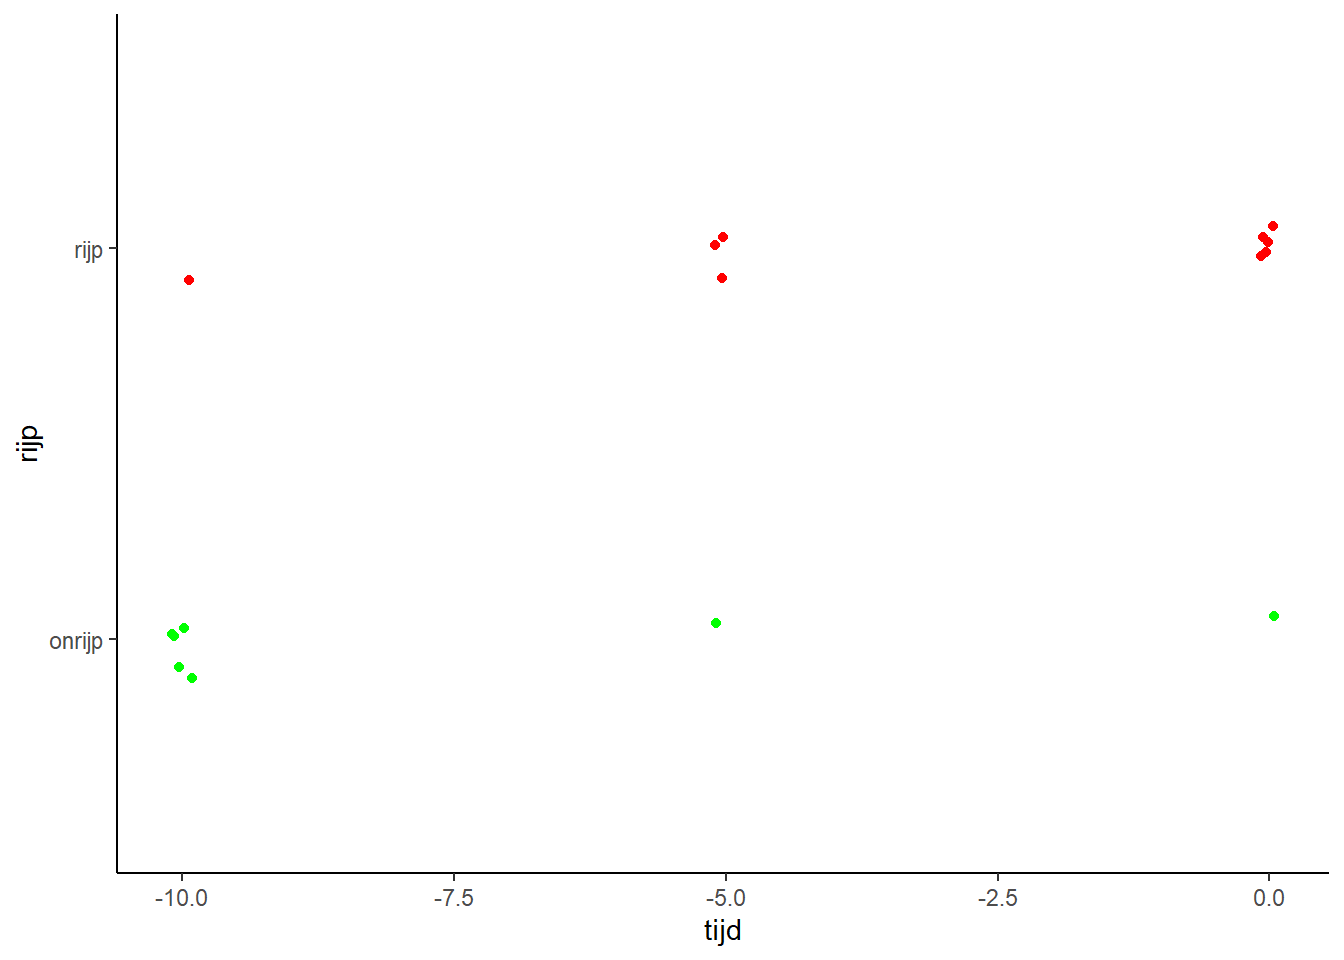
\includegraphics{hfst2_logregr_files/figure-latex/unnamed-chunk-13-1.pdf}

Voor de duidelijkheid zijn de individuele punten iets verspreid
weergegeven (via \texttt{geom\_jitter()}). Met wat toevoegingen
(\texttt{color\ =\ rijp},
\texttt{scale\_color\_manual(values\ =\ c("green",\ "red"))}) zijn de
rijpe waarden rood en onrijpe waarden weer groen.

Nu hebben we op de x-as geen categoriën, maar een continue schaal.
Zouden we nu iets met een regressie kunnen doen? Het antwoord is ja.

Met hetzelfde \emph{generalized linear model} kunnen we ook regressies
uitvoeren:

\begin{Shaded}
\begin{Highlighting}[]
\NormalTok{fit2 <-}\StringTok{ }\KeywordTok{glm}\NormalTok{(rijp ~}\StringTok{ }\NormalTok{tijd, }\DataTypeTok{family =} \KeywordTok{binomial}\NormalTok{(), }\DataTypeTok{data =} \NormalTok{tomaat_num)}
\end{Highlighting}
\end{Shaded}

Het enige verschil met de vorige analyse is dat we van de variabele tijd
\textbf{geen} factor maken.

Kijken wat de uitkomst is met de functie \texttt{Anova()}:

\begin{Shaded}
\begin{Highlighting}[]
\KeywordTok{Anova}\NormalTok{(fit2)}
\end{Highlighting}
\end{Shaded}

\begin{verbatim}
## Analysis of Deviance Table (Type II tests)
## 
## Response: rijp
##      LR Chisq Df Pr(>Chisq)  
## tijd   5.9506  1    0.01471 *
## ---
## Signif. codes:  0 '***' 0.001 '**' 0.01 '*' 0.05 '.' 0.1 ' ' 1
\end{verbatim}

Fractie rijpe vruchten lijkt dus inderdaad te veranderen met de tijdstip
van plukken.

Met de functie \texttt{summary()} krijg je de geschatte parameters van
het statistisch model te zien:

\begin{Shaded}
\begin{Highlighting}[]
\KeywordTok{summary}\NormalTok{(fit2)}
\end{Highlighting}
\end{Shaded}

\begin{verbatim}
## 
## Call:
## glm(formula = rijp ~ tijd, family = binomial(), data = tomaat_num)
## 
## Deviance Residuals: 
##     Min       1Q   Median       3Q      Max  
## -2.0802  -0.7021   0.4941   0.6254   1.7443  
## 
## Coefficients:
##             Estimate Std. Error z value Pr(>|z|)  
## (Intercept)   2.0416     1.1143   1.832   0.0669 .
## tijd          0.3316     0.1597   2.077   0.0378 *
## ---
## Signif. codes:  0 '***' 0.001 '**' 0.01 '*' 0.05 '.' 0.1 ' ' 1
## 
## (Dispersion parameter for binomial family taken to be 1)
## 
##     Null deviance: 21.930  on 15  degrees of freedom
## Residual deviance: 15.979  on 14  degrees of freedom
## AIC: 19.979
## 
## Number of Fisher Scoring iterations: 4
\end{verbatim}

Het model is een rechte lijn die de y-as (die de \textbf{log-odd-waarde}
aangeef!) snijdt op 2,0416 en een richtingscoëfficiënt heeft van 0.3316.

Voor de tomatenteler is het van belang vanaf welk tijdstip het
waarschijnlijk is dat een minimale fractie tomaten (zeg 25\% rijp is).
Daarvoor hebben we het betrouwbaarheidsinterval nodig.

Met ggplot kunnen we gemakkelijk het betrouwbaarheidsinterval plotten,
en tegelijkertijd de minimale fractie rijpheid aangeven:

\begin{Shaded}
\begin{Highlighting}[]
\NormalTok{tomaat_num %>%}\StringTok{ }
\StringTok{  }\KeywordTok{ggplot}\NormalTok{(}\KeywordTok{aes}\NormalTok{(tijd, rijp)) +}\StringTok{ }
\StringTok{  }\KeywordTok{geom_point}\NormalTok{(}\DataTypeTok{alpha=}\FloatTok{0.2}\NormalTok{, }\DataTypeTok{size =} \DecValTok{2}\NormalTok{) +}
\StringTok{  }\KeywordTok{geom_smooth}\NormalTok{(}\DataTypeTok{method=}\NormalTok{glm, }\DataTypeTok{method.args =} \KeywordTok{list}\NormalTok{(}\DataTypeTok{family =} \KeywordTok{binomial}\NormalTok{())) +}
\StringTok{  }\KeywordTok{ylab}\NormalTok{(}\StringTok{"Fractie rijp"}\NormalTok{) +}
\StringTok{  }\KeywordTok{geom_hline}\NormalTok{(}\DataTypeTok{yintercept =} \FloatTok{0.25}\NormalTok{, }\DataTypeTok{color =} \StringTok{"blue"}\NormalTok{, }\DataTypeTok{linetype =} \StringTok{"dashed"}\NormalTok{)}
\end{Highlighting}
\end{Shaded}

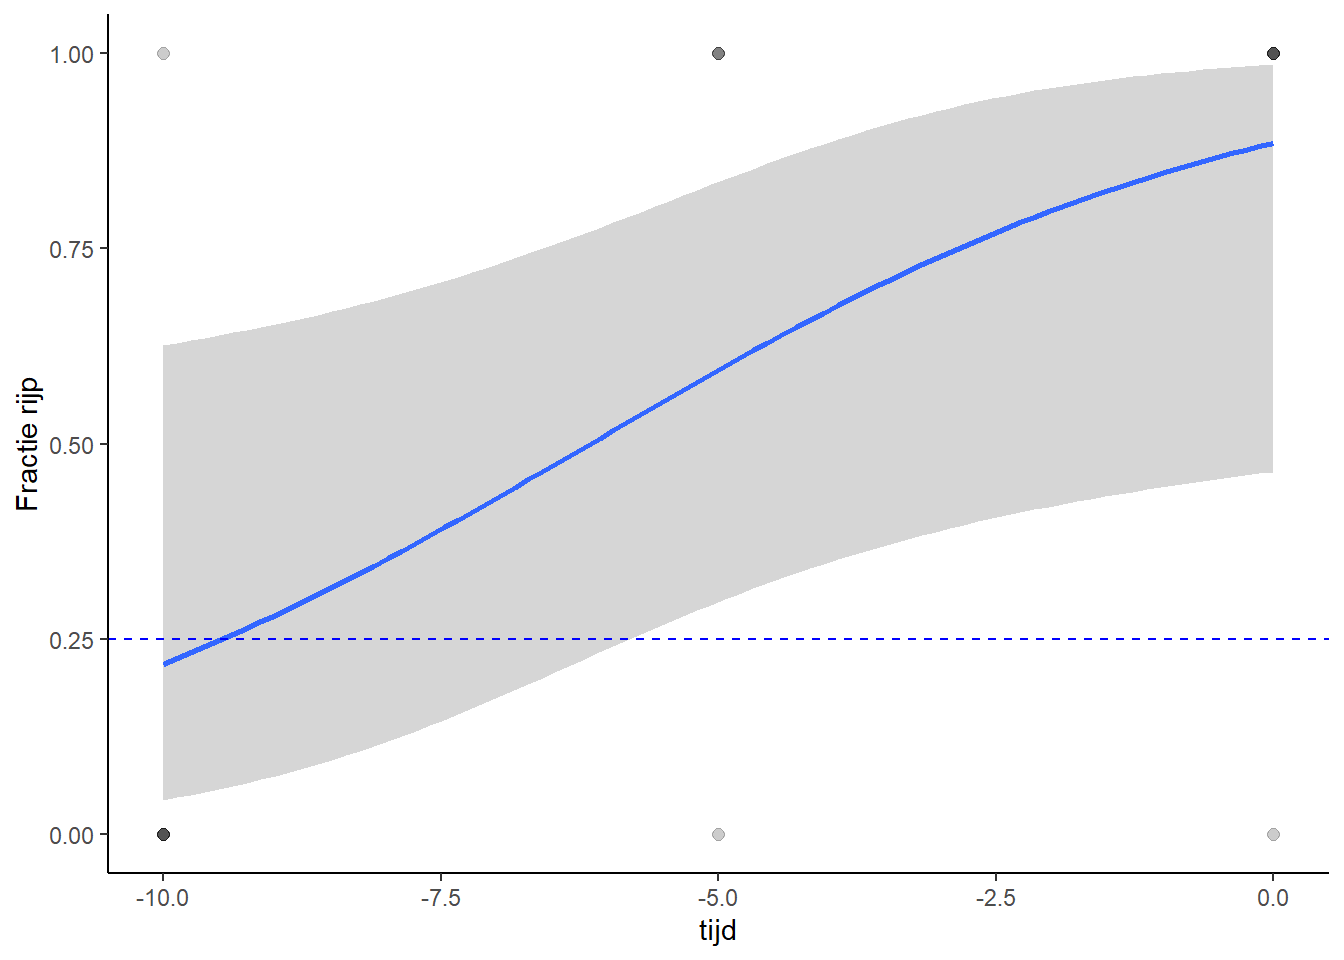
\includegraphics{hfst2_logregr_files/figure-latex/unnamed-chunk-17-1.pdf}

\begin{Shaded}
\begin{Highlighting}[]
  \KeywordTok{theme}\NormalTok{(}\DataTypeTok{legend.position =} \StringTok{"none"}\NormalTok{) }
\end{Highlighting}
\end{Shaded}

\begin{verbatim}
## List of 1
##  $ legend.position: chr "none"
##  - attr(*, "class")= chr [1:2] "theme" "gg"
##  - attr(*, "complete")= logi FALSE
##  - attr(*, "validate")= logi TRUE
\end{verbatim}

Je ziet nu de typische S-vorm van een logistisch regressie. Bij vijf
dagen eerder oogsten zit de teler dus nog veilig.

\BeginKnitrBlock{exercise}
\protect\hypertarget{exr:guppies}{}{\label{exr:guppies} }Guppies

Pitkow \emph{et al.} (1960) onderzocht het effect van tijdsduur
blootstelling aan lage temperatuur op de overleving van guppies. Hij
stelde steeds 40 guppies bloot aan water van 5°C, voor 3, 8, 12 of 18
minuten.

\begin{itemize}
\tightlist
\item
  Download de data van BB (guppies.xlsx)
\item
  Zet de data uit in een grafiek.
\item
  Voer een logistische regressie uit.
\item
  Wat zijn je conclusies?
\end{itemize}
\EndKnitrBlock{exercise}

\section{LT50}\label{lt50}

De afkorting LT50 is een begrip uit de toxicologie en staat voor de
``mediaan letale tijd'' (tijd tot aan de dood). Wat breder
geïnterpreteerd staat het voor de waarde van de verklarende factor
waarbij de kans op succes 0,5 is.

In principe kan je met behulp van de \emph{estimates} van het logistisch
model uitrekenen bij welke waarde je LT50 bereikt, maar er is
(natuurlijk) een gemakkelijke functie voor: \texttt{dose.p()}.

Deze functie zit in de package MASS. Nu is het punt met \textbf{MASS}
dat er een paar functies in zitten met dezelfde naam als functies in de
package \textbf{tidyverse}. Om te voorkomen dat deze functies
overschreven worden, kan je een functie ook oproepen zonder de hele
library op te roepen. Dat doe je op de volgende manier:

\texttt{MASS::dose.p(fit,\ p=0.5)}

Die dubbele dubbele punt betekent dat je vanuit de package MASS de
functie dose.p oproept.

In bovenstaande functie staat fit voor het GLM-model, en het argument p
geeft aan voor welke kans je de waarde voor de verklarende factor wilt
weten.

Als voorbeeld weer de tomaten. De teler wilt weten op welk moment 75\%
van de tomaten rijp zijn:

\begin{Shaded}
\begin{Highlighting}[]
\NormalTok{MASS::}\KeywordTok{dose.p}\NormalTok{(fit2, }\DataTypeTok{p=}\FloatTok{0.75}\NormalTok{)}
\end{Highlighting}
\end{Shaded}

\begin{verbatim}
##              Dose       SE
## p = 0.75: -2.8435 2.349679
\end{verbatim}

Bij 2,84 dagen voor oogsten is gemiddeld 75\% van de tomaten rijp. De
standaardfout van deze schatting is 2,35

\BeginKnitrBlock{exercise}
\protect\hypertarget{exr:LT50}{}{\label{exr:LT50} }LT50

\begin{itemize}
\tightlist
\item
  Welke log-odd hoort bij LT50?
\end{itemize}
\EndKnitrBlock{exercise}

\BeginKnitrBlock{exercise}
\protect\hypertarget{exr:MASS}{}{\label{exr:MASS} }MASS

\begin{itemize}
\tightlist
\item
  installeer de package MASS
\item
  Bereken de LG50 voor het voorbeeld van de Guppies.
\end{itemize}
\EndKnitrBlock{exercise}

\chapter{Chikwadraattoets}\label{chikwadraattoets}

\BeginKnitrBlock{ABD}
\begin{itemize}
\tightlist
\item
  Lees \emph{chapter} 8 (\emph{Fitting probability models to frequency
  data})
\item
  Lees \emph{section} 9.4 (\emph{The \(\chi^2\) contigency test})
\end{itemize}
\EndKnitrBlock{ABD}

Dit hoofdstuk gaat, net als de vorige hoofdstukken, over nominale data.
Heb je meer dan twee categoriën, dan kan je geen binomiale toets meer
gebruiken. Daarvoor is de Chi-kwadraattoets ontwikkeld. Deze ben je al
tegengekomen in de output van de verschiltoets voor fracties
(\texttt{prop.test()}). Nu gaan we hier dieper op in.

\section{Chi-kwadraattoets op
aanpassing}\label{chi-kwadraattoets-op-aanpassing}

Met de Chi-kwadraattoets op aanpassing (\emph{goodness of fit}) kan
onderzocht worden of de waargenomen aantallen een bepaalde verdeling
volgen. Er wordt getoetst of de gevonden frequenties in het onderzoek
overeenkomen met een verwachte verdeling tussen die frequenties op basis
van bijvoorbeeld:

\begin{itemize}
\tightlist
\item
  eerdere waarnemingen
\item
  een theoretisch model (bijvoorbeeld uit de genetica)
\item
  kennis van de hele populatie (representativiteit).
\end{itemize}

De Chi-kwadraattoets op aanpassing toetst of het aannemelijk is dat de
aantallen in een bepaalde steekproef overeenkomen met de theoretisch te
verwachten waarden. De toets maakt onderscheid tussen `kleine'
verschillen en `grote' verschillen: worden de verschillen veroorzaakt
door het toeval (verschillen zijn klein) of zal de conclusie zijn dat de
verdeling in de steekproef afwijkt van de verwachte verdeling
(verschillen zijn voldoende groot, ofwel significant).

Als voorbeeld data van jullie kruisingsexperiment met kolen:

\begin{tabular}{l|r}
\hline
fenotype & frequentie\\
\hline
glad-groen & 3\\
\hline
groen-gekruld & 14\\
\hline
rood-glad & 10\\
\hline
rood-gekruld & 37\\
\hline
\end{tabular}

De onderzoeksvraag was of de gevonden verdeling de verwachte verdeling
volgt als rood en gekruld dominanten eigenschappen zijn, en de kruising
Mendeliaanse overerving volgt.

De hypotheses zijn dan:

\begin{itemize}
\tightlist
\item
  H\textsubscript{0}: de verdeling volgt de theoretische verdeling.
\item
  H\textsubscript{1}: de verdeling volgt niet de theoretische verdeling.
\end{itemize}

\section{Voorwaarden}\label{voorwaarden}

De Chi-kwadraattoets is een afgeleide van de F-verdeling, welke weer een
afgeleide is van de normale verdeling. Dat werkt goed zolang de kans op
een bepaalde frequentie niet te klein is. Dat kan je checken met de
\textbf{regel van Cochran}:

\begin{itemize}
\tightlist
\item
  Alle verwachte frequenties zijn groter of gelijk aan 1
\item
  Het percentage cellen met verwachte frequenties kleiner dan 5 is
  minder dan 20\%
\end{itemize}

Als niet aan deze voorwaarden voldaan wordt, heb je de volgende opties:

\begin{itemize}
\tightlist
\item
  Categoriën samenvoegen (zodat de gecombineerde frequenties boven de
  drempelwaarde komen)
\item
  De H\textsubscript{0} simuleren door middel van heel veel
  berekeneningen (wat heel gemakkelijk gaat in R)
\end{itemize}

\BeginKnitrBlock{exercise}
\protect\hypertarget{exr:cochran}{}{\label{exr:cochran}
}Kruisingsexperiment:

\begin{itemize}
\tightlist
\item
  Test of de data van de kruisingsproef voldoet aan de regels van
  Cochran
\end{itemize}
\EndKnitrBlock{exercise}

\section{Chi-kwadraattoets in R}\label{chi-kwadraattoets-in-r}

Met de functie \texttt{chisq.test()} voor je de Chi-kwadraattoets uit
(in dit geval voor de data van de kruisingsproef):

\begin{Shaded}
\begin{Highlighting}[]
\KeywordTok{chisq.test}\NormalTok{(df$frequentie, }\DataTypeTok{p=}\KeywordTok{c}\NormalTok{(}\DecValTok{1}\NormalTok{/}\DecValTok{16}\NormalTok{, }\DecValTok{3}\NormalTok{/}\DecValTok{16}\NormalTok{, }\DecValTok{3}\NormalTok{/}\DecValTok{16}\NormalTok{,  }\DecValTok{9}\NormalTok{/}\DecValTok{16}\NormalTok{))}
\end{Highlighting}
\end{Shaded}

Als argumenten zijn de gevonden frequentie en de verwachte kansverdeling
(als een vector) gegeven.

Hieronder staat de uitkomst:

\begin{verbatim}
## 
##  Chi-squared test for given probabilities
## 
## data:  df$frequentie
## X-squared = 0.94444, df = 3, p-value = 0.8147
\end{verbatim}

X-squared staat voor de Chi-kwadraatwaarde, df voor het aantal
vrijheidsgraden en p-value voor de overschrijdingskans onder de
H\textsubscript{0}.

In dit geval is \(p>0.05\), dus we verwerpen de H\textsubscript{0} niet
(met \(\alpha=0.05\)). We kunnen dus niet de aanname van Mendeliaanse
overerving verwerpen. Of met andere woorden: de gevonden frequentie is
niet significant afwijkend van de voorspelde frequentie volgens
Mendeliaanse overerving.

NB: de kansverdeling over de verschillende categoriën (argument
\textbf{p} in de functie) moet bij elkaar opgeteld precies 1 zijn. Dat
kan simpel met de volgende code
\texttt{p=df\$verwach/sum(df\$verwacht)}. Alternatief is om als extra
argument \texttt{rescale.p\ =\ TRUE} te gebruiken. Dan berekent R
automatisch de kansverdeling.

\BeginKnitrBlock{exercise}
\protect\hypertarget{exr:plantenkwekers}{}{\label{exr:plantenkwekers}
}Enquête plantenkwekers:

In 2008 teelde 33\% van de Nederlandse snijbloementelers als
hoofdproduct roos, 29\% chrysant, 25\% tulp, de overige 13\% andere
soorten. In 2008 werd een enquête gehouden onder 200 Nederlandse
snijbloementelers. Daarvan teelden er 70 roos als hoofdgewas, 52
chrysant, 49 tulp, en de overige 29 andere soorten:
\EndKnitrBlock{exercise}

\begin{tabular}{l|r|r}
\hline
Hoofdgewas & Aantal telers in enquête & Percentage kwekers\\
\hline
Roos & 70 & 33\\
\hline
Chysant & 49 & 29\\
\hline
Tulp & 52 & 25\\
\hline
Overig & 29 & 13\\
\hline
\end{tabular}

De vraag is of de enquête representatief is voor de Nederlandse telers
(met andere woorden de respondenten volgen dezelfde verdeling als de
verdeling van kwekers in Nederland over de verschillende hoofdgewassen).

\begin{itemize}
\tightlist
\item
  Beschrijf de H\textsubscript{0} en de H\textsubscript{1}.
\item
  Test of aan de regel van Cochran wordt voldaan.
\item
  Voer een Chi-kwadraattoets uit (voer data direct in in R, of maak
  eerst een Excelbestand).
\item
  Wat is je conclusie
\end{itemize}

\section{Poisonverdeling}\label{poisonverdeling}

Met een Chi-kwadraattoets test je de gevonden frequentieverdeling ten
opzichte van een theoretische verdeling. Een veel voorkomende verdeling
is de Poisonverdeling. Deze verdeling is vernoemd naar
\href{https://nl.wikipedia.org/wiki/Sim\%C3\%A9on_Poisson}{Siméon
Poisson}.

Net als de binomiale verdeling gaat het hier om discrete data. Het geeft
ook de kans op x-aantal voorvallen. Het verschil met de binomiale
verdeling is dat je niet uitgaat van een bepaald aantal herhalingen
(zoals de voorbeelden met een dobbelsteen), maar uitgaat van een
\emph{richting} oneindig aantal herhalingen (n) met een \emph{richting}
oneindig kleine kans (p) waarbij \(n*p=\lambda\). Het teken \(\lambda\)
(de Griekse letter \emph{Lambda}) staat voor het gemiddelde aantal
voorvallen.

Klinkt ingewikkeld? Bekijk het voorbeeld (met figuren!) van de
rekolonisatie door spinnen in het boek aandachten.

Gelukkig heeft R een simpele functie om de kansverdeling uit te rekenen.
Als voorbeeld \emph{example 8.6} uit het boek:

\begin{itemize}
\tightlist
\item
  Sterven organismen random uit in de geschiedenis van het leven?
\end{itemize}

Raup en Sepkoski (1982) hebben data verzameld van mariene invertebraten
en per tijdsblok aangegeven hoeveel families er uitstierven:

\begin{tabular}{r|r}
\hline
aantal\_uitstervingen & frequentie\\
\hline
0 & 0\\
\hline
1 & 13\\
\hline
2 & 15\\
\hline
3 & 16\\
\hline
4 & 7\\
\hline
5 & 10\\
\hline
6 & 4\\
\hline
7 & 2\\
\hline
8 & 1\\
\hline
9 & 2\\
\hline
10 & 1\\
\hline
11 & 1\\
\hline
12 & 0\\
\hline
13 & 0\\
\hline
14 & 1\\
\hline
15 & 0\\
\hline
16 & 2\\
\hline
17 & 0\\
\hline
18 & 0\\
\hline
19 & 0\\
\hline
20 & 1\\
\hline
\end{tabular}

De vraag is nu of uitsterven gezien kan worden als random proces in de
tijd, of dat er juist momenten zijn waarbij relatief veel dieren
uitsterven (massa-extincties).

De H\textsubscript{0} is dat uitsterven een random proces is, dus een
Poissonverdeling volgt. De H\textsubscript{1} is dat uitsterven niet de
Poissonverdeling volgt.

In R kunnen we gemakkelijk de verwachte waarden per tijdsvak uitrekenen
als de H\textsubscript{0} waar is.

De eerste stap is het gemiddeld aantal uitstervingen per tijdsvak te
berekenen (\(\lambda\) in de functie voor de Poissonverdeling).
Bovenstaande tabel is een frequentietabel, in dertien tijdsvakken is
bijvoorbeeld 1 mariene invertebraatgroep uitgestorven. Om het gemiddelde
per tijdsvak te berekenen moeten we iedere regel net zo vaak meetellen
als de frequentie aangeeft. Dat noem je een gewogen gemiddelde:

\begin{Shaded}
\begin{Highlighting}[]
\NormalTok{lambda <-}\StringTok{ }\KeywordTok{weighted.mean}\NormalTok{(df$aantal_uitstervingen, df$frequentie)}
\NormalTok{lambda}
\end{Highlighting}
\end{Shaded}

\begin{verbatim}
## [1] 4.210526
\end{verbatim}

Met deze waarde kunnen we verwachte frequentie voor ieder aantal
uitstervingen per tijdvak berekenen:

\begin{Shaded}
\begin{Highlighting}[]
\NormalTok{df$verwacht <-}\StringTok{ }\KeywordTok{dpois}\NormalTok{(df$aantal_uitstervingen, }\DataTypeTok{lambda =} \NormalTok{lambda)*}\KeywordTok{sum}\NormalTok{(df$frequentie)}
\end{Highlighting}
\end{Shaded}

Met \texttt{dpois()} bereken je de dichtheid voor ieder aantal. Als je
dat vermenigvuldigt met het totale aantal tijdvakken (de som van de
frequenties) dan krijg je de verwachte verdeling van aantal
uitstervingen over het totaal aantal tijdblokken (76 in dit geval).

Nu kunnen we de daadwerkelijke en de verwachte verdeling weergeven in
een grafiek:

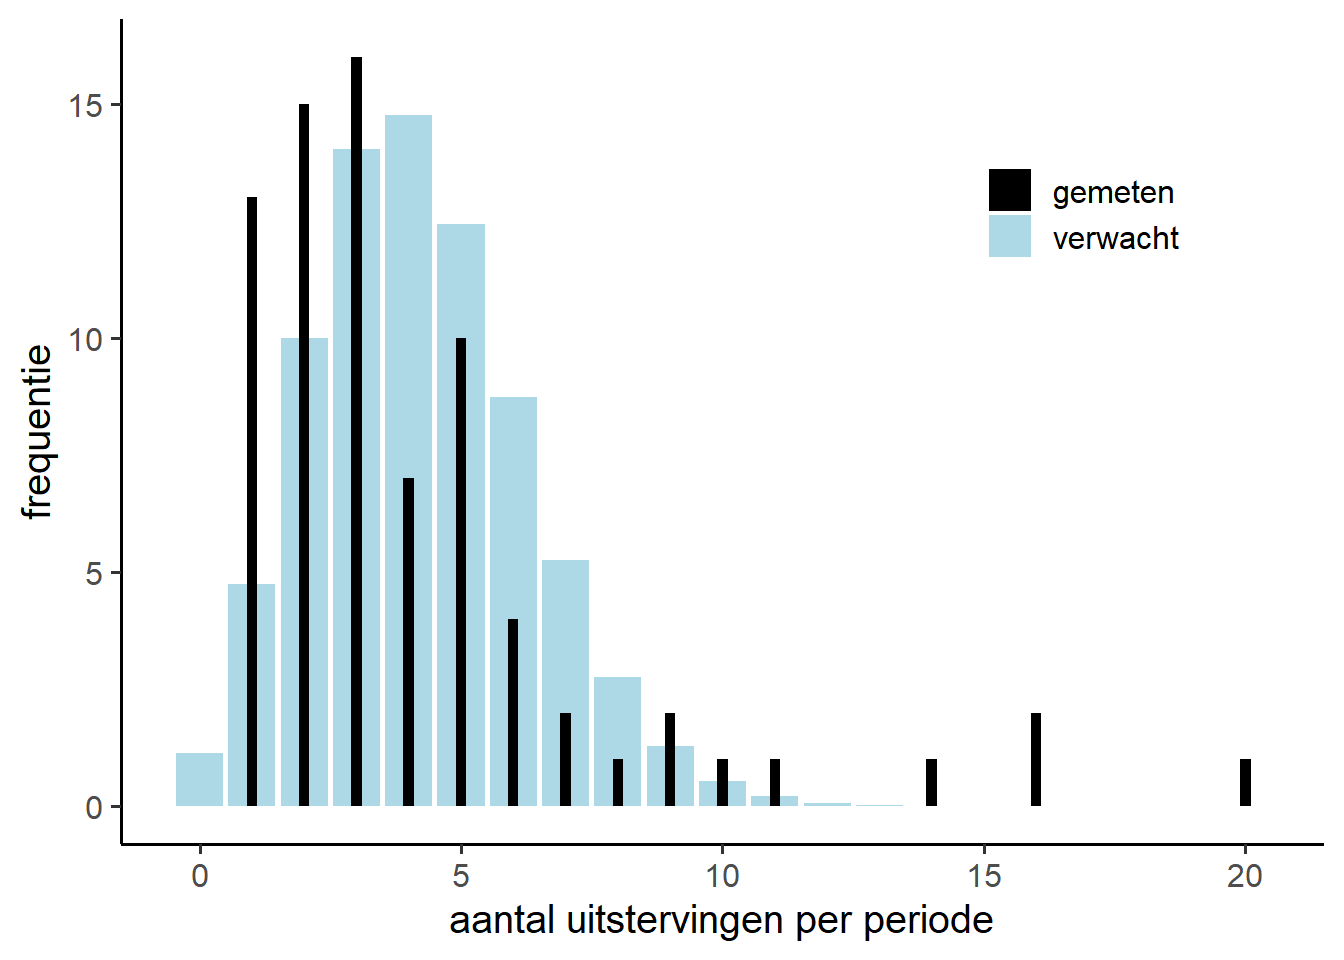
\includegraphics{hfst3_chi_aanpassing_files/figure-latex/unnamed-chunk-9-1.pdf}

Je kan in de grafiek al zien dat de werkelijke verdeling anders loopt
dan de Poissonverdeling. Hoe waarschijnlijk is het nu om minstens zo'n
afwijking t.o.v. de Poissonverdeling te vinden als H\textsubscript{0}
klopt?

We hebben nu een gevonden en een verwachte frequentievedeling, dus
kunnen we daar een Chi-kwadraattoets op loslaten.

Eerst de regel van Cochran toepassen:

\begin{itemize}
\tightlist
\item
  E\textsubscript{i}\textless{} 1?
\item
  Aantal E\textsubscript{i} \textless{} 5 \textgreater{} 20\% van
  E\textsubscript{i}'s?
\end{itemize}

Elf cellen hebben een verwachte frequentie kleiner dan 1, en 15 cellen
een verwachte frequentie kleiner dan 5 (dat is meer dan 20\% van 21
cellen). Dus we kunnen de Chi-kwadraattoets niet toepassen.

\subsection{Optie 1: categoriën
samenvoegen}\label{optie-1-categoriuxebn-samenvoegen}

In het boek passen ze optie 1 toe: categorieën samenvoegen. Je krijgt
dan de volgende verdeling:

\begin{tabular}{l|r|r}
\hline
categorie & frequentie & verwacht\\
\hline
a & 13 & 5.876068\\
\hline
b & 15 & 9.996501\\
\hline
c & 16 & 14.030177\\
\hline
d & 7 & 14.768607\\
\hline
e & 10 & 12.436722\\
\hline
f & 4 & 8.727524\\
\hline
g & 2 & 5.249639\\
\hline
h & 9 & 4.914760\\
\hline
\end{tabular}

Bijbehorende Chi-kwadraattoets:

\begin{Shaded}
\begin{Highlighting}[]
\KeywordTok{chisq.test}\NormalTok{(df_cat$frequentie, }\DataTypeTok{p=}\NormalTok{df_cat$verwacht, }\DataTypeTok{rescale.p =} \OtherTok{TRUE}\NormalTok{)}
\end{Highlighting}
\end{Shaded}

\begin{verbatim}
## 
##  Chi-squared test for given probabilities
## 
## data:  df_cat$frequentie
## X-squared = 23.95, df = 7, p-value = 0.001163
\end{verbatim}

NB: bovenstaande output is een fractie anders dan de uitwerking in het
boek. De reden is dat de verwachte frequenties berekend zijn op basis
van het geschatte gemiddelde aantal uitstervingen per tijdvak. Hiermee
snoep je een vrijheidsgraad op. Wil je het helemaal netjes aanpakken,
dan moet je handmatig aangeven hoeveel vrijheidsgraden de
Chikwadraatverdeling heeft onder de H\textsubscript{0}:

\begin{Shaded}
\begin{Highlighting}[]
\NormalTok{fit <-}\StringTok{ }\KeywordTok{chisq.test}\NormalTok{(df_cat$frequentie, }\DataTypeTok{p=}\NormalTok{df_cat$verwacht, }\DataTypeTok{rescale.p =} \OtherTok{TRUE}\NormalTok{)}
\KeywordTok{pchisq}\NormalTok{(fit$statistic, }\DataTypeTok{df=}\DecValTok{6}\NormalTok{, }\DataTypeTok{lower.tail =} \OtherTok{FALSE}\NormalTok{)}
\end{Highlighting}
\end{Shaded}

\begin{verbatim}
##    X-squared 
## 0.0005334918
\end{verbatim}

\subsection{Optie twee: simuleren}\label{optie-twee-simuleren}

Optie twee is de verdeling onder de H\textsubscript{0} te simuleren. Dat
kan met dezelfde functie \texttt{chisq.test()}, met als extra argument
\texttt{simulate.p.value\ =\ TRUE}:

\begin{Shaded}
\begin{Highlighting}[]
\KeywordTok{chisq.test}\NormalTok{(df$frequentie, }\DataTypeTok{p=}\NormalTok{df$verwacht, }
           \DataTypeTok{rescale.p =} \OtherTok{TRUE}\NormalTok{,}\DataTypeTok{simulate.p.value =} \OtherTok{TRUE}\NormalTok{)}
\end{Highlighting}
\end{Shaded}

\begin{verbatim}
## 
##  Chi-squared test for given probabilities with simulated p-value (based
##  on 2000 replicates)
## 
## data:  df$frequentie
## X-squared = 711152, df = NA, p-value = 0.0004998
\end{verbatim}

\BeginKnitrBlock{exercise}
\protect\hypertarget{exr:extinction}{}{\label{exr:extinction} }Uitsterven

\begin{itemize}
\tightlist
\item
  Downdload de data van BB (``uitsterven.xlsx'').
\item
  Voer de Chi-kwadraattoets uit op de orinele data (wetende dat het niet
  voldoet aan de regel van Cochran).
\item
  Voer nu de toets uit waarbij de de kansverdeling onder de
  H\textsubscript{0} gesimuleerd wordt.
\item
  Vergelijk de gevonden p-waarden. Neemt de fout van de eerste soort toe
  of af? Leg uit.
\end{itemize}
\EndKnitrBlock{exercise}

\section{Chikwadraattoets op
onafhankelijkheid}\label{chikwadraattoets-op-onafhankelijkheid}

Zoals je in \emph{section} 9.4 van het boek kan lezen, kan je de
Chikwadraattoets ook gebruiken als je wilt testen of twee nominale
variabele afhankelijk van elkaar zijn. Met andere woorden: heeft
categorie van de ene variabele effect op frequentieverdeling over de
categorieën van de andere variabele.

Als voorbeeld \emph{Example} 9.4 uit het boek. Onderzoekers hebben het
vermoeden dat vissen die geïnfecteerd zijn door een parasitaire worm een
grotere kans hebben om gegeten te worden door reigers omdat ze vaker aan
het oppervlak zwemmen. Lafferty en Morris (1996) testten deze hypothese
door vissen met drie niveaus van infectiegraad in een groot bassin te
laten zwemmen, en te tellen hoeveel van welke groep gepredeerd werd:

\begin{tabular}{l|l|r}
\hline
gegeten & infectiegraad & frequentie\\
\hline
niet gegeten & niet & 1\\
\hline
niet gegeten & licht & 10\\
\hline
niet gegeten & zwaar & 37\\
\hline
wel gegeten & niet & 49\\
\hline
wel gegeten & licht & 35\\
\hline
wel gegeten & zwaar & 9\\
\hline
\end{tabular}

Bovenstaande manier is een goede manier om de data uit \emph{Table}
9.4-1 in bijv. Excel te zetten.

De volgende hypotheses worden getest met de Chikwadraattoets op
onafhankelijkheid:

\begin{itemize}
\tightlist
\item
  H\textsubscript{0}: Infectiegraad en gegeten worden zijn onafhankelijk
\item
  H\textsubscript{1}: Infectiegraad en gegeten worden zijn niet
  onafhankelijk
\end{itemize}

De Chikwadraattoets op onafhankelijkheid kan op verschillende manieren
data verwerken:

\begin{itemize}
\tightlist
\item
  als \texttt{table()} output (heb je gezien bij de krekeldata in jaar
  1)
\item
  als `lange' tabel met op iedere regel een waarneming (je hebt dan 141
  regels!)
\item
  als matrix (gaan we hier niet doen)
\end{itemize}

Voor de eerste twee methoden moet je eerst de tabel `lang' maken. Daar
is in tidyverse een simpele functie voor \texttt{uncount()}:

\begin{Shaded}
\begin{Highlighting}[]
\KeywordTok{library}\NormalTok{(tidyverse)}
\NormalTok{df_lang <-}\StringTok{ }\NormalTok{df %>%}\StringTok{ }
\StringTok{  }\KeywordTok{uncount}\NormalTok{(frequentie)}
\end{Highlighting}
\end{Shaded}

Dan kan je de de Chikwadraattoets op onafhankelijkheid uitvoeren:

\begin{Shaded}
\begin{Highlighting}[]
\KeywordTok{chisq.test}\NormalTok{(df_lang$gegeten, df_lang$infectiegraad)}
\end{Highlighting}
\end{Shaded}

\begin{verbatim}
## 
##  Pearson's Chi-squared test
## 
## data:  df_lang$gegeten and df_lang$infectiegraad
## X-squared = 69.756, df = 2, p-value = 7.124e-16
\end{verbatim}

In principe kan je deze toets ook uitvoeren als je meer dan twee
nominale variabelen hebt.

\section{Extra opgaven}\label{extra-opgaven}

Gebruik bij onderstaande opgaven uit het boek R. Ga dus niet zelf met de
hand de Chikwadraatwwaarde uitrekenen, en overschrijdingskans opzoeken
in een tabel. Daar hebben we tegenwoordig computers voor!

\BeginKnitrBlock{exercise}
\protect\hypertarget{exr:chiboek}{}{\label{exr:chiboek} }\emph{Practise
problems}

Maak de volgende *Practise problems chapter 8 (vanaf blz. 225):

\begin{itemize}
\tightlist
\item
  1, 2, 3
\end{itemize}

Maak de volgende *Practise problems chapter 9 (vanaf blz. 258):

\begin{itemize}
\tightlist
\item
  2, 7

  \EndKnitrBlock{exercise}
\end{itemize}

\chapter{Clusteranalyse}\label{clusteranalyse}

\BeginKnitrBlock{ABD}
\EndKnitrBlock{ABD}

we leven in het `big data'-tijdperk. Iedereen (op een enkele
fanatiekeling na) die regelmatig gebruik maakt van internet draagt zijn
steentje bij aan de informatieberg. Deze informatie wordt gebruikt om
``profielen'' aan te maken. Daarmee krijgen we gepersonificeerde
reclame, nieuwsberichten, zoekresultaten, etc. Hiervoor is statistiek
nodig: multivariate analyses.

Multivariaat slaat op het aantal \textbf{respons}variabelen. Tot nu toe
hadden we te maken met één responsvariabele waarvan we de variatie
wilden verklaren aan de hand van een of meerdere \textbf{verklarende}
variabelen. Nu hebben we te maken met meerdere (soms wel duizenden)
responsvariabelen (bijv. hoe vaak je bepaalde websites gezocht hebt, of
bepaalde zoektermen voorkwamen in je zoekopdrachten). Vandaar de term
\textbf{multi}variaat.

Binnen de ecologie wordt al lang met multivariate data gewerkt, vooral
binnen de vegetatiekunde. De responsvariabelen zijn dan de abundantie
van de verschillende plantensoorten per plot. Een onderzoeksvraag kan
zijn welke plots op elkaar lijken en welke van elkaar verschillen.

Met de opkomst van \emph{metagenomics} hebben we niet alleen voor
planten, maar ook voor andere organismen (vooral microbiologie) enorme
datasets met multivariate data.

Deze week en volgende week gaan jullie aan de slag met multivariate
data. We behandelen twee technieken:

\begin{itemize}
\tightlist
\item
  Clustering (deze les)
\item
  MANOVA (volgende les)
\end{itemize}

Clustering is, zoals de naam al zegt, het clusteren van multivariate
data. MANOVA staat voor \emph{Multivariate Analysis of Variance}, een
soort van ANOVA met meerdere responsvariabelen.

\begin{quote}
NB De bijbehorende powerpoint is tentamenstof. De volgende paragrafen
over clustering is in ontwikkeling, en geen tentamenstof (maar
natuurlijk wel heel interessant!).
\end{quote}

\section{Twee manieren van clusteren}\label{twee-manieren-van-clusteren}

Jullie zijn met het vak biotechnologie al een vorm van clusteren
tegengekomen: de fylogenetische boom (\textbf{fylogram}), een voorbeeld
van een \textbf{dendrogram}. Deze manier van clusteren wordt
\textbf{hierarchisch} genoemd.

Een andere manier van clusteren

\chapter{Overzicht toetsen}\label{overzicht-toetsen}

\BeginKnitrBlock{ABD}
\EndKnitrBlock{ABD}

\chapter{MANOVA}\label{manova}

intro

\end{document}
